\section{Experiments and Results}
\label{sec:experiments}

%%PA: let's be careful about overclaiming here, and make it clear
%%up-front that we consider a simulated PR2 robot.  

%%PA: how about structuring this section a bit more explicitly:
%% \subsection{Experimental Setup} with further subsections
%% {Simulation Environment for Knot Tying} and {Benchmark} where the
%% benchmark clearly mentions the labeling process as well as how
%% initial states are generated including the test states
%% \subsection{Experiments}  and here we describe the different
%% methods we consider;  

\subsection{Experimental Setup}
We evaluate the greedy policy and two beam search lookahead policies using the Willow Garage PR2 robot in a simulation environment, for the task of tying an overhand knot.

\subsubsection{Demonstrations}
We use the set of demonstrations collected by \citet{Schulmanetal_ISRR2013} for their rope-tying experiments.
These demonstrations were collected in the real world and consist of 148 pairs of point clouds and gripper trajectories.
The point clouds were collected using an RGBD camera and then filtered based on color to remove the green background of the table, and leave only the point cloud representation of the rope.
The gripper trajectories were recorded kinesthetically, from human-guided demonstrations that move the robot's grippers to tie a knot.
The dataset contains demonstrations for the three steps of tying an overhand knot, as well as demonstrations to recover from rope states that could lead to failure cases.

\subsubsection{Simulation Environment for Knot Tying} 
The training, validation, and evaluation of the trained policy are run in simulation.
The simulation environment uses Bullet Physics~\cite{Bullet_Physics} as the physics engine.
The rope is simulated as a linked chain of capsules with bending and torsional constraints.

\subsubsection{Benchmark}
For the labeled examples \labelset{} used to train our \mmql{} model, we distinguish between expert- (i.e. human-) labeled examples and automatically generated leave-one-out labeled examples.
In both cases, the examples consists of point clouds, each associated with an optimal action.
The point clouds in these examples consist of sequences of complete task executions, from a randomly drawn initial rope configuration to a knot (Section~\ref{subsec:labeledex}.
The radomly drawn initial rope states are perturbed configurations of randomly chosen initial rope states from the demonstrations.
The process of perturbing a rope state consists of selecting five uniformly-spaced points along the rope and dragging each in a random direction for a random radius of within 15 cm.
The randomly generated initial rope configurations mentioned hereafter are drawn from this distribution.
For the expert-labelled examples, the expert does not see the execution of all the actions to select the optimal action.
Instead, the actions are ranked in increasing order of registration cost with respect to the current state and the expert selects an action as optimal if that action makes some progress on tying the rope.
The leave-one-out labeled examples are generated as outlined in Section~\ref{subsec:lool}. \al{Do we need to say more about this in here?}
The benchmark used is the success rate of running the trained policy in simulation on 500 randomly drawn initial rope configurations. 
We define success as tying an overhand knot in a sequence of 5 or fewer actions.

\subsection{Experiments}
We evaluate the success rate using the following policies when using the expert-labeled and leave-one-out labeled examples: greedy, one-step lookahead with width 10, and two-step lookahead with width 5.
\subsubsection{Expert-labeled Examples}
For this evaluation, 1000 expert-labeled examples are used.
For each of these policies, the optimization hyperparameters $C$, $D$ and $F$ are first tuned via holdout validation, using a holdout set of 100 randomly drawn initial rope states. For this case, the best-performing hyperparameters we found are $C=2$, $D=1$ and $F=1$.
Using this hyperparameters, we optimize the weights and then run each of the three policies on the evaluation set, which consists of 500 randomly drawn initial rope states.
% TODO: Add in what the hyperparameters are, once we decide on them
As a baseline comparison, we also evaluate using the nearest neighbor policy presented in \citet{Schulmanetal_ISRR2013}.
Their policy chooses the action associated with the state that has the smallest bidirectional registration cost with respect to the current state.
The success rates obtained under these policies are summarized in Table~\ref{table:performance}. Note that our best results surpass the baseline by 26.4\%.
% TODO: Add more analysis of the results, e.g. 1-10 and 2-5 lookahead perform approximately equally well

\begin{table}
  \centering
  \begin{tabular}{lc}
    \toprule
      Policy & Test Accuracy\\
    \midrule
      Nearest neighbor \cite{Schulmanetal_ISRR2013} & 68.8\% \\
    \midrule
      Greedy & 85.6\% \\
      Lookahead (depth 1, width 10) & 93.6\% \\
      Lookahead (depth 2, width 5) & 95.2\% \\
    \bottomrule
  \end{tabular}
  \caption{Success rate of tying a knot using the expert-labeled examples.}
  \label{table:performance}
\end{table}

The approximate values of the states for the 500 evaluated runs in the validation set are plotted in Figure~\ref{fig:values} as a function of time steps 1 through 5.
%TODO: shift plot from 1 to 5
Observe that the state values are generally increasing; we expect this since the Bellman constraints in our formulation pushes states closer to the goal to have higher values.
Also, recall that the state value of the tied knot is close to zero, which is visible in the figure (Equation~\ref{eq:bellman_goal_constr}).
For most of the runs, the policy is able to reach the goal state in 3 steps, which is optimal since the expert took a minimun of three actions to tie a knot.

\begin{figure}
  \centering
  \begin{subfigure}[b]{0.9\linewidth}
    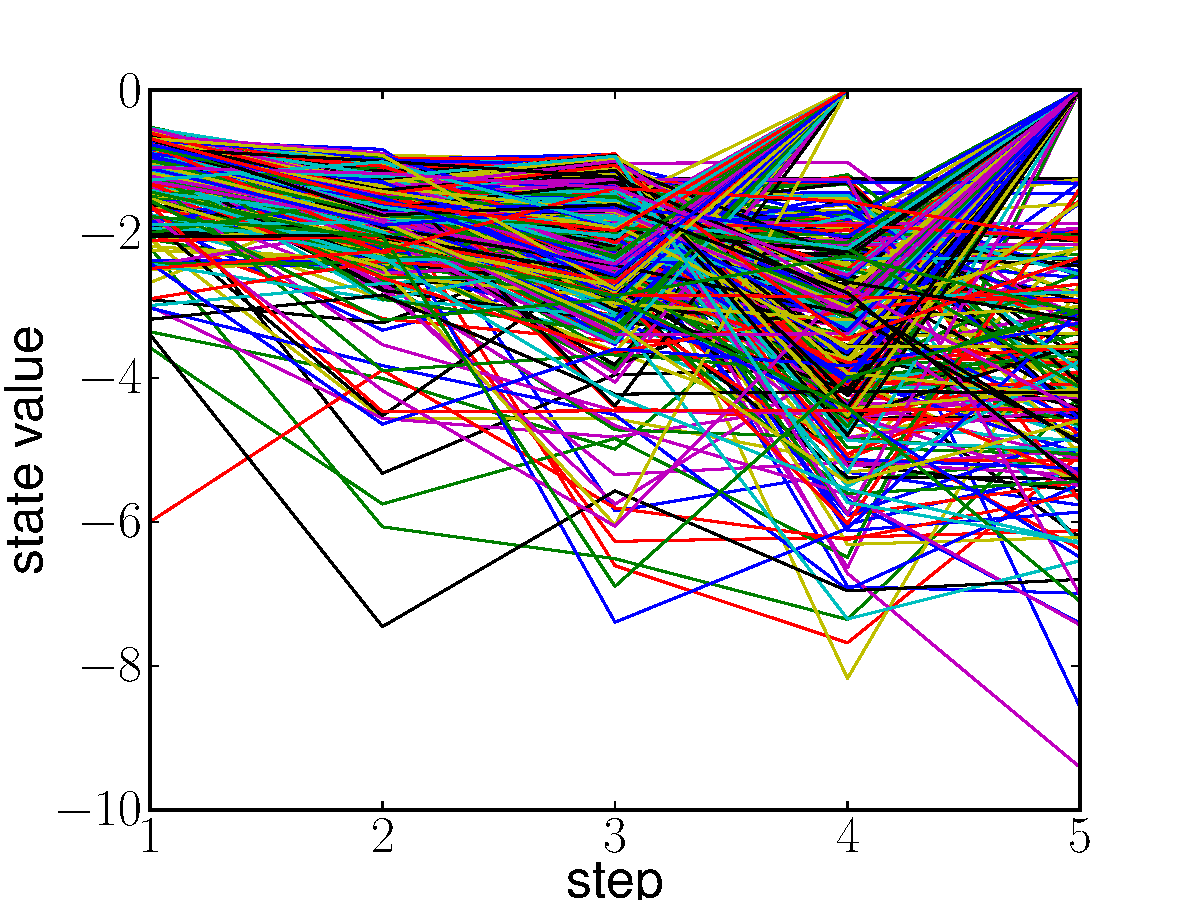
\includegraphics[width=\textwidth]{figures/state_value_baseline.pdf}
    \caption{baseline}
    \label{fig:value_baseline}
  \end{subfigure}
  \begin{subfigure}[b]{0.9\linewidth}
    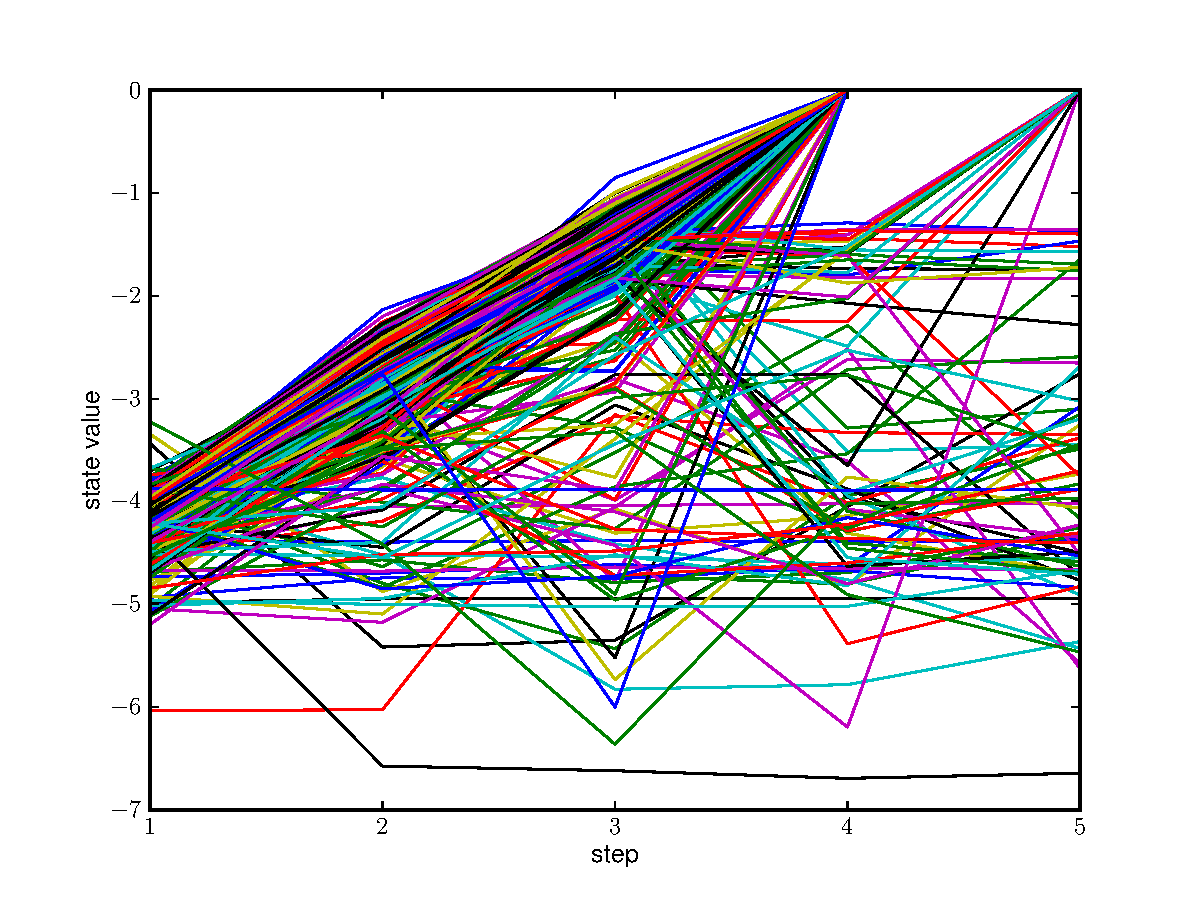
\includegraphics[width=\textwidth]{figures/state_value_greedy.pdf}
    \caption{greedy}
    \label{fig:value_greedy}
  \end{subfigure}
  \begin{subfigure}[b]{0.9\linewidth}
    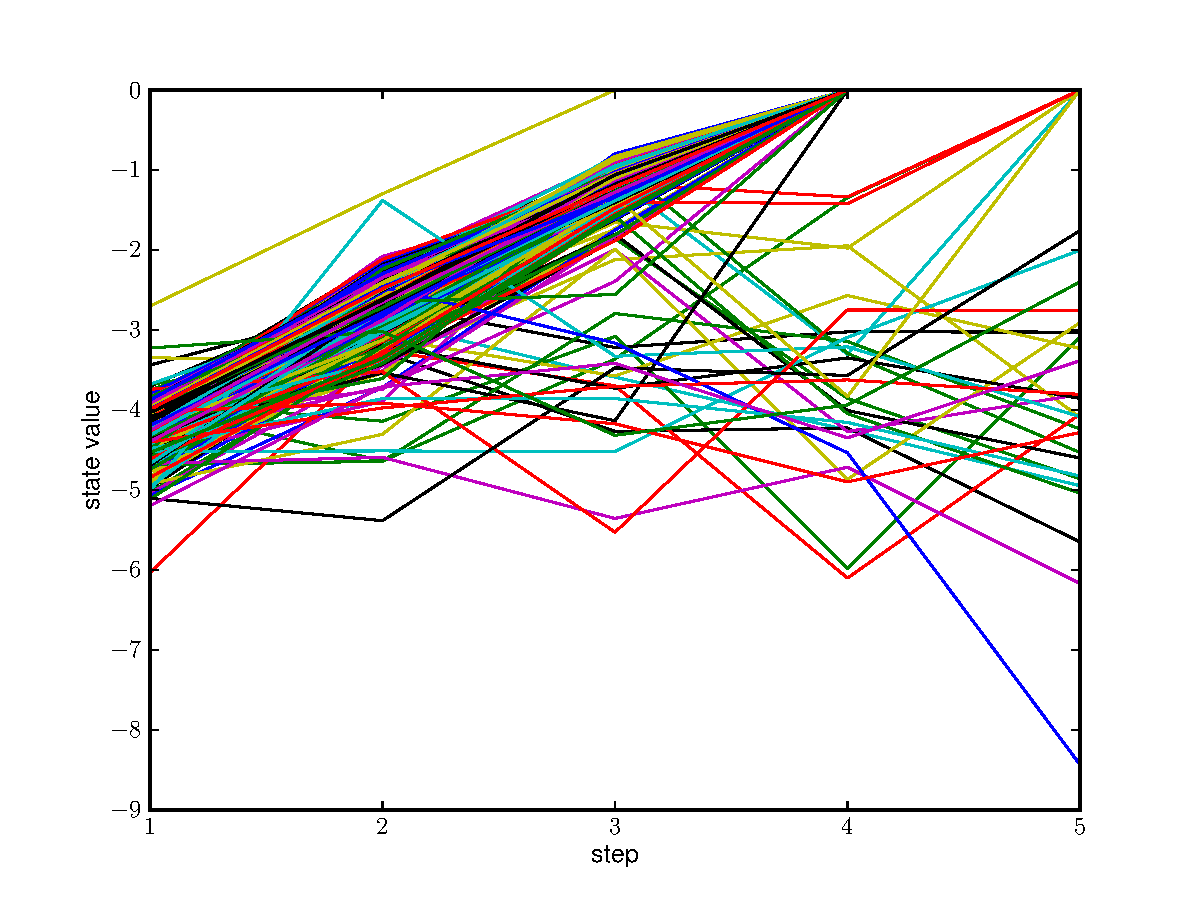
\includegraphics[width=\textwidth]{figures/state_value_lookahead2-5.pdf}
    \caption{lookahead (depth 2, width 5)}
    \label{fig:value_lookahead_2}
  \end{subfigure}
  \caption{State values as a function of time steps under different policies}\label{fig:values}
\end{figure}



We also study the relation between the number of expert-labeled examples and the success rate for each of the four policies, including the nearest-neighbor baseline policy.
These success rates are shown in Figure~\ref{fig:number_examples}.
The success rate of the baseline policy is a constant, since the nearest neighbor policy doesn't use the expert-labeled examples.
As expected, the success rate increases as more labeled-examples are used.
%TODO: Mention that there are diminishing returns as you increase the number of expert examples (I assume the graph will look like that)

\begin{figure}[h!]
  \centering
    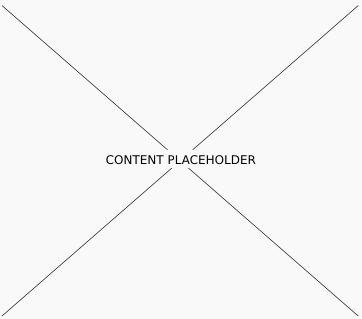
\includegraphics[width=0.9\linewidth]{figures/placeholder.png}
  \caption{Success rates as a function of the number of expert-labelled examples for the four policies}
  \label{fig:number_examples}
\end{figure}

\subsubsection{Leave-One-Out Labeled Examples}

After holdout validation and evaluation, done in the same manner as our main
experiment, we find that using a leave-one-out labeled example set achieves a
performance of XX\%, a drop of XX\% from our supervised result.
%\et{It feels difficult to do further analysis without an actual number here. I'll save this
%for later, if that's alright with everyone.}
